\documentclass[11pt,a4paper]{article}
\usepackage[margin=2.2cm]{geometry}
\usepackage{amsmath,amssymb}
\usepackage{booktabs}
\usepackage{graphicx}
\usepackage{hyperref}

% Figures and tables are written by notebooks/exercise_4.ipynb
\graphicspath{{../results/exercise_4/}}
\newcommand{\res}{../results/exercise_4}

\title{EP2 -- Exercise 4\\One spherical collapse, three numerical formulations}
\author{Victor Roberto Soares da Silva}
\date{}

\begin{document}
\maketitle

\section{Model and equations}

We follow the smooth-dark-energy, shear-free limit of Pace, Meyer \& Bartelmann~\cite{pace2017}, as fixed in the Lecture~8 notes~\cite{notes8}.
The background is flat $\Lambda$CDM (EdS for $\Omega_{m0}=1$) with radiation neglected at all epochs:
\begin{equation}
  E^2(a) = \Omega_{m0}a^{-3} + 1-\Omega_{m0},\qquad
  \Omega_m(a) = \frac{\Omega_{m0}a^{-3}}{E^2},\qquad
  A_H = 2 + \frac{d\ln H}{dN} = 2 - \frac{3}{2}\Omega_m(a),
\end{equation}
with $N=\ln a$, $X_N = dX/dN$, $\vartheta = \nabla_x\cdot v/(aH)$ and $g = 1/\delta$ (inverse overdensity, not the growth rate).
The three nonlinear systems and the linear equation are
\begin{align}
  \text{A:}\quad & \delta_{NN} + A_H\delta_N - \frac{4}{3}\frac{\delta_N^2}{1+\delta} - \frac{3}{2}\Omega_m\delta(1+\delta) = 0, \\
  \text{B:}\quad & \delta_N = -(1+\delta)\vartheta, \qquad \vartheta_N = -A_H\vartheta - \frac{\vartheta^2}{3} - \frac{3}{2}\Omega_m\delta, \\
  \text{C:}\quad & g_N = g(1+g)\vartheta, \qquad \vartheta_N = -A_H\vartheta - \frac{\vartheta^2}{3} - \frac{3\Omega_m}{2g}, \\
  \text{linear:}\quad & \delta_{L,NN} + A_H\delta_{L,N} - \frac{3}{2}\Omega_m\delta_L = 0 .
\end{align}
A is integrated as the first-order pair $(\delta,\delta_N)$, B as $(\delta,\vartheta)$ and C as $(g,\vartheta)$, each with its own right-hand side and its own call to the integrator.
Algebraic equivalence was checked at $10^3$ random states ($10^{-5}<\delta<10^{8}$): differentiating B's continuity equation reproduces A's $\delta_{NN}$, and C at $g=1/\delta$ reproduces $g_N=-\delta_N/\delta^2$ and B's $\vartheta_N$, to $\lesssim 10^{-14}$.
The three independent trajectories agree to $\lesssim10^{-9}$ until just before collapse (Fig.~\ref{fig:traj}).

\begin{figure}[h]
  \centering
  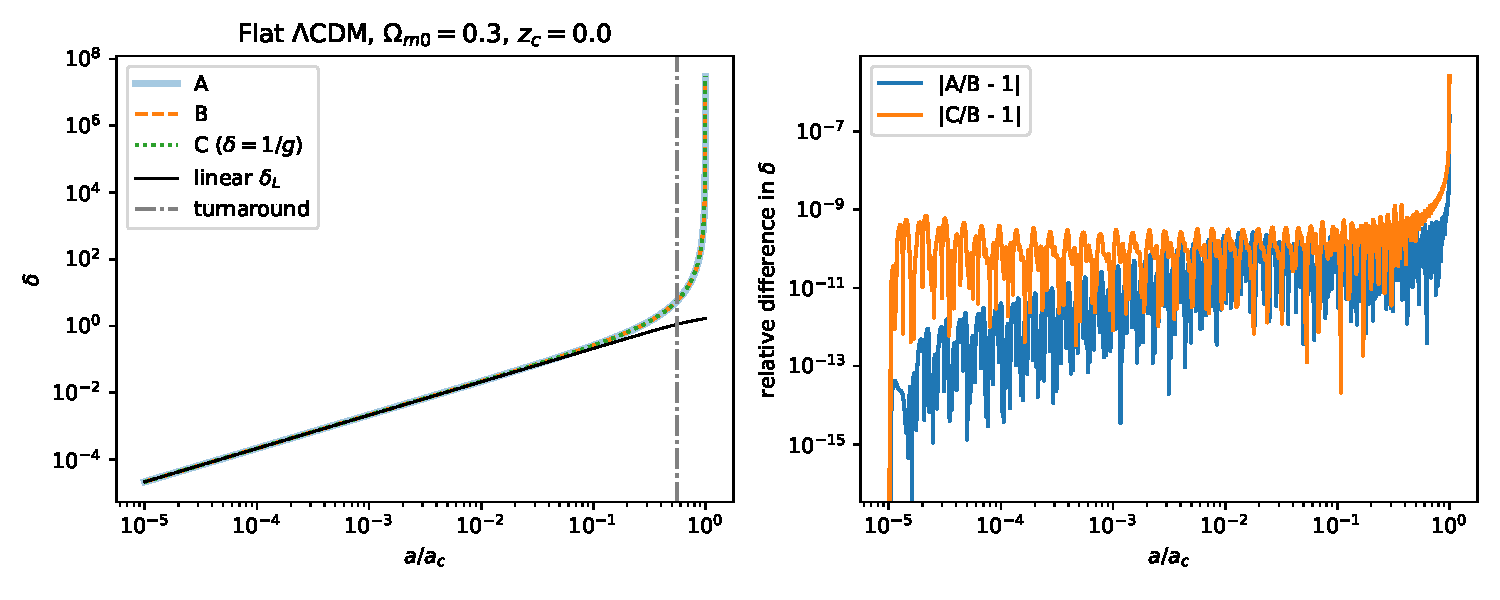
\includegraphics[width=\linewidth]{fig_trajectories.pdf}
  \caption{Left: $\delta(a)$ from A, B, C (same $\delta_i$) and the linear $\delta_L$; flat $\Lambda$CDM, $\Omega_{m0}=0.3$, $z_c=0$. Right: relative differences between the independent integrations.}
  \label{fig:traj}
\end{figure}

\section{Initial conditions, events and shooting}

For a trial $\delta_i$ at $a_i \ll a_c$ (growing mode, notes eq.~6.6):
\begin{equation}
  \delta_{N,i} = f_i\delta_i,\qquad \vartheta_i = -\frac{f_i\delta_i}{1+\delta_i},\qquad g_i = \delta_i^{-1},\qquad
  \delta_{L,i} = \delta_i,\quad \delta_{L,N,i} = f_i\delta_i,
\end{equation}
where $f_i = d\ln D/d\ln a$ at $a_i$ is taken from the Exercise~1 growth ODE started at $a_i/100$ ($1-f_i \lesssim 10^{-9}$ for $a_i\le10^{-3}$).

\begin{itemize}
  \item \textbf{Collapse event} (terminal): $\delta=\delta_\infty$ for A and B, $g=\epsilon$ for C. The integration stops there and never crosses the singular endpoint.
  \item \textbf{Turnaround event}: $d\ln R/dN = 1+\vartheta/3 = 0$, i.e.\ $\vartheta=-3$ (A uses $\vartheta=-\delta_N/(1+\delta)$, C uses $\delta = 1/g$); $\zeta_\mathrm{ta} = 1+\delta(a_\mathrm{ta})$.
  \item \textbf{Shooting}: Brent's method on $F(\delta_i) = N_\mathrm{event}(\delta_i) - \ln a_c$. The bracket starts at $[0.9,1.1]\times 1.686\,D(a_i)/D(a_c)$ and is widened until $F$ changes sign. Relative tolerance on $\delta_i$: $10^{-13}$.
  \item $\delta_c = \delta_L(a_c)$ from the linear solution with the tuned $\delta_i$.
  \item \textbf{Defaults}: $a_i = 10^{-5}$, \texttt{scipy.integrate.solve\_ivp} with \texttt{DOP853}, \texttt{rtol}$=10^{-10}$, \texttt{atol}$=10^{-14}$, $\delta_\infty = 10^8$, $\epsilon=10^{-8}$.
\end{itemize}
Table~\ref{tab:out} lists the required outputs for $z_c=0$, including brackets, number of iterations and event residuals.

\begin{table}[h]
  \centering
  \caption{Required outputs for $z_c=0$ (default settings). $\ln(a_\mathrm{ev}/a_c)$ is the event residual.}
  \label{tab:out}
  \resizebox{\linewidth}{!}{\input{\res/tab_outputs_zc0.tex}}
\end{table}

\section{Virial prescription}

The same prescription is applied to the outputs of A, B and C (notes Section~3.3).
With $y=R_\mathrm{vir}/R_\mathrm{ta}$ and
\begin{equation}
  \lambda_\mathrm{ta} = \frac{\rho_\Lambda}{\rho_\mathrm{sph,ta}} = \frac{\Omega_\Lambda(a_\mathrm{ta})}{\Omega_m(a_\mathrm{ta})\,\zeta_\mathrm{ta}},
  \qquad 4\lambda_\mathrm{ta}y^3 - 2(1+\lambda_\mathrm{ta})y + 1 = 0 ,
\end{equation}
we take the root in $(0,1/2]$: the cubic equals $+1$ at $y=0$ and $-\lambda_\mathrm{ta}/2$ at $y=1/2$, and this root tends continuously to $y=1/2$ as $\lambda_\mathrm{ta}\to0$ (EdS).
Using the formal-collapse epoch,
\begin{equation}
  \Delta_{\mathrm{vir},m}(a_c) = \zeta_\mathrm{ta}\left(\frac{a_c}{a_\mathrm{ta}}\right)^3 y^{-3},\qquad
  \Delta_{\mathrm{vir},c}(a_c) = \Omega_m(a_c)\,\Delta_{\mathrm{vir},m}(a_c).
\end{equation}

\section{EdS benchmarks}

Table~\ref{tab:eds} compares with $\delta_c = \frac{3}{20}(12\pi)^{2/3} = 1.68647$, $a_\mathrm{ta}/a_c = 2^{-2/3}$, $\zeta_\mathrm{ta}=(3\pi/4)^2$, $\Delta_{\mathrm{vir},m}=18\pi^2$, at four collapse redshifts.
$\zeta_\mathrm{ta}$ is recovered to $\sim10^{-10}$. $a_\mathrm{ta}/a_c$ ($+6.7\times10^{-5}$) and $\Delta_{\mathrm{vir},m}$ ($-2.0\times10^{-4}$) have the same error at every $z_c$: it is the finite-threshold bias, since the event fires slightly before the true collapse.
$\delta_c$ has, in addition to this bias ($\approx -6.7\times10^{-5}$), the initial-epoch error $\propto\delta_i\propto a_i/a_c$ (Section~\ref{sec:conv}), which explains its small drift with $z_c$ at fixed $a_i$. No threshold was tuned to match any single benchmark.

\begin{table}[h]
  \centering
  \caption{EdS validation: relative errors with respect to the exact values (default settings).}
  \label{tab:eds}
  \resizebox{\linewidth}{!}{\input{\res/tab_eds.tex}}
\end{table}

The finite-threshold bias scales as $\delta_\infty^{-1/2}$ (Fig.~\ref{fig:thr}). This follows from the cycloid (notes eq.~2.6): near $\eta=2\pi$, $R\propto(t_c-t)^{2/3}$, so $\delta\propto(t_c-t)^{-2}$ and the event at $\delta_\infty$ comes early by $\Delta t/t_c\propto\delta_\infty^{-1/2}$.
With $\epsilon=1/\delta_\infty$, A, B and C give identical errors: the bias belongs to the event, not to the formulation.

\begin{figure}[h]
  \centering
  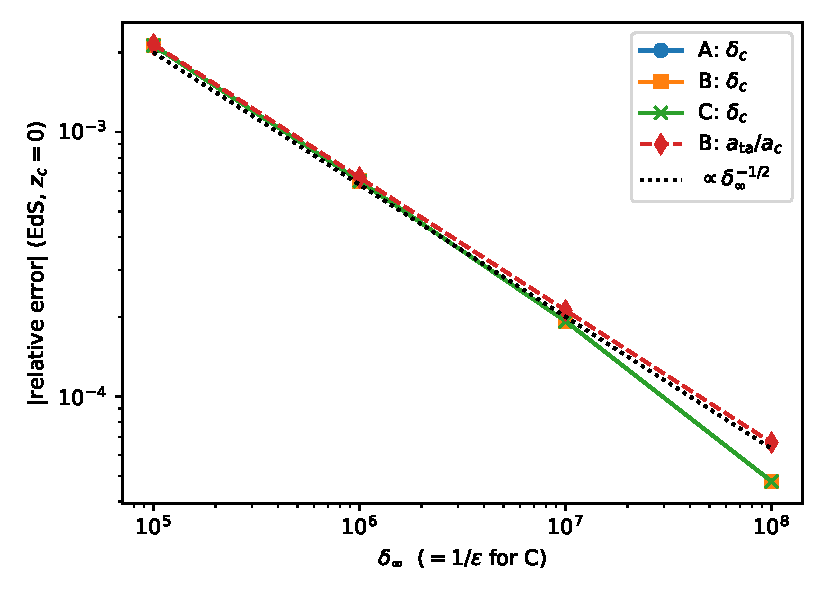
\includegraphics[width=0.55\linewidth]{fig_threshold.pdf}
  \caption{EdS, $z_c=0$: relative error in $\delta_c$ (A, B, C) and $a_\mathrm{ta}/a_c$ (B) versus the event threshold.}
  \label{fig:thr}
\end{figure}

\section{Flat $\Lambda$CDM grid}

Figure~\ref{fig:grid} and Table~\ref{tab:grid} show $\Omega_{m0}\in\{0.2,0.3,0.4\}$, $\Omega_{\Lambda0}=1-\Omega_{m0}$, $z_c\in\{0,1,2\}$ (curves use a finer $z_c$ step of $0.25$).
Over the full grid the spread between A, B and C is $\le2\times10^{-10}$ in $\delta_c$, $\zeta_\mathrm{ta}$ and $\Delta_{\mathrm{vir},m}$.

\begin{figure}[h]
  \centering
  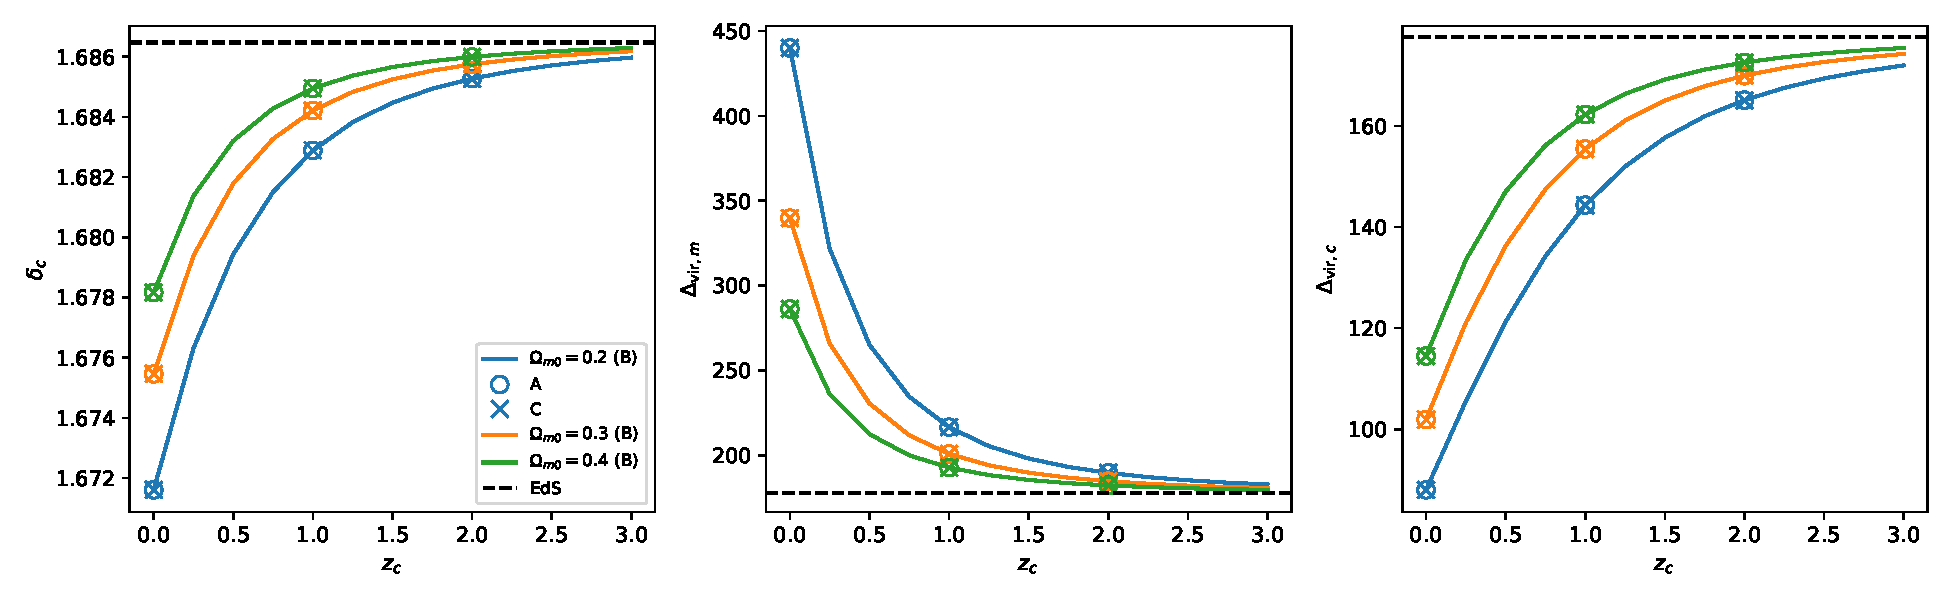
\includegraphics[width=\linewidth]{fig_grid.pdf}
  \caption{$\delta_c$, $\Delta_{\mathrm{vir},m}$ and $\Delta_{\mathrm{vir},c}$ versus $z_c$. Lines: B; open markers: A and C at $z_c=0,1,2$; dashed: EdS.}
  \label{fig:grid}
\end{figure}

\begin{table}[h]
  \centering
  \caption{Flat $\Lambda$CDM grid (formulation B; A and C agree to $\le2\times10^{-10}$).}
  \label{tab:grid}
  \input{\res/tab_grid.tex}
\end{table}

\begin{table}[h]
  \centering
  \caption{Factor decomposition: $\Delta_{\mathrm{vir},m}/18\pi^2 = [\zeta_\mathrm{ta}/\zeta^\mathrm{EdS}_\mathrm{ta}]\times[(a_c/a_\mathrm{ta})^3/4]\times(2y)^{-3}$, and $\Delta_{\mathrm{vir},c}/\Delta_{\mathrm{vir},m}=\Omega_m(a_c)$.}
  \label{tab:dec}
  \resizebox{\linewidth}{!}{\input{\res/tab_decomposition.tex}}
\end{table}

\paragraph{Roles of the different ingredients} (Table~\ref{tab:dec}).
\begin{itemize}
  \item \textbf{Growth.} $\Lambda$ slows the linear growth and the nonlinear collapse by almost the same amount, so $\delta_c$ decreases by less than $1\%$ (lowest $\Omega_{m0}$, $z_c=0$: $0.991\,\delta_c^\mathrm{EdS}$).
  \item \textbf{Turnaround.} The sphere turns around denser ($\zeta_\mathrm{ta}$ up to $1.34\times$ EdS) and earlier relative to collapse ($a_\mathrm{ta}/a_c<2^{-2/3}$), so the background dilutes more until $a_c$ (factor up to $1.62$). These are the two largest factors in $\Delta_{\mathrm{vir},m}$.
  \item \textbf{Virial prescription.} The $\Lambda$ potential energy gives $y<1/2$: a smaller, denser virialized halo (factor up to $1.14$).
  \item \textbf{Reference density.} $\Delta_{\mathrm{vir},m}$ rises above $18\pi^2$ while $\Delta_{\mathrm{vir},c}=\Omega_m(a_c)\Delta_{\mathrm{vir},m}$ falls below it, because $\Omega_m(a_c)<1$: the same halo shows opposite trends for the two conventions.
\end{itemize}
At high $z_c$ matter dominates and all quantities approach the EdS lines.

\section{Convergence and failure modes}
\label{sec:conv}

Flat $\Lambda$CDM, $\Omega_{m0}=0.3$, $z_c=0$. One setting is changed at a time and $\delta_i$ is retuned in every run.
The reference is B with \texttt{rtol}$=10^{-12}$, \texttt{atol}$=10^{-16}$ ($\delta_c = 1.6754603968$, $\Delta_{\mathrm{vir},m} = 339.714231$, $\Delta_{\mathrm{vir},c}=101.914269$); it shares $a_i$ and the threshold with the defaults, so those rows measure differences with respect to the default, not to the exact answer.

\begin{table}[h]
  \centering
  \caption{Relative change of $\delta_c$ with respect to the reference, cross-formulation difference and worst event residual. Threshold setting: $\delta_\infty$ / $\epsilon$; tolerances: \texttt{rtol} / \texttt{atol}; ``loose atol'' uses \texttt{rtol}$=10^{-10}$; ``method'' uses \texttt{rtol}$=10^{-6}$.}
  \label{tab:convdc}
  \resizebox{\linewidth}{!}{\input{\res/tab_convergence_delta_c.tex}}
\end{table}

\begin{table}[h]
  \centering
  \caption{Same as Table~\ref{tab:convdc} for $\Delta_{\mathrm{vir},m}$.}
  \label{tab:convD}
  \input{\res/tab_convergence_Dvir.tex}
\end{table}

\begin{itemize}
  \item \textbf{All formulations.} (i) Threshold bias $\propto\delta_\infty^{-1/2}$; from this scaling the error left at $\delta_\infty=10^8$ is $\approx6\times10^{-5}$ in $\delta_c$ and $\approx2\times10^{-4}$ in $\Delta_\mathrm{vir}$, as in EdS. It is the dominant error at the default settings. (ii) Initial epoch: eq.~(6.6) is the growing mode only to first order in $\delta_i$, so the $\delta_c$ error scales as $\delta_i\propto a_i$ ($2.4\times10^{-3}$ at $a_i=10^{-3}$, $2.2\times10^{-4}$ at $10^{-4}$). $\zeta_\mathrm{ta}$ and $\Delta_\mathrm{vir}$ do not move with $a_i$: the shooting absorbs the initial error in the nonlinear run, while $\delta_c$ inherits it through $\delta_L$. Event residuals stay $\lesssim10^{-13}$, so the root search is never the limitation.
  \item \textbf{A.} $\delta$ and $\delta_N$ both diverge and the source contains $\delta_N^2/(1+\delta)$. Early on $\delta\sim10^{-5}$, so \texttt{atol} must be $\ll\delta_i$; \texttt{atol}$=10^{-6}$ gives $6\times10^{-5}$ in $\delta_c$.
  \item \textbf{B.} Same \texttt{atol}--$\delta_i$ sensitivity as A ($5\times10^{-5}$); $\delta$ and $|\vartheta|$ diverge at collapse.
  \item \textbf{C.} $g$ runs from $\sim5\times10^4$ down to $\epsilon$, so \texttt{atol} must be $\ll\epsilon$, otherwise the event $g=\epsilon$ is not resolved: \texttt{atol}$=10^{-6}$ gives $2\times10^{-3}$, the largest error of all. C is also the most sensitive to a loose \texttt{rtol} and a lower-order integrator ($10^{-5}$ with RK45), as the $1/g$ source and $\vartheta$ still diverge.
\end{itemize}
With tight settings A, B and C agree to $\sim10^{-10}$, far below the threshold and $a_i$ effects. We do not reproduce the statement that C is less noisy~\cite{pace2017}: with adaptive step control and event location, C is as precise as A and B at tight settings and less robust at loose ones.

\begin{thebibliography}{9}
  \bibitem{pace2017} F.~Pace, S.~Meyer and M.~Bartelmann, ``On the implementation of the spherical collapse model for dark energy models,'' JCAP \textbf{10}, 040 (2017), arXiv:1708.02477.
  \bibitem{notes8} T.~Castro, \emph{Lecture 8 Notes: Spherical Collapse and Halo Abundances}, Numerical Cosmology, IFUSP; Sections 2, 3, 6 and 7.
  \bibitem{scipy} P.~Virtanen et al., ``SciPy 1.0: fundamental algorithms for scientific computing in Python,'' Nature Methods \textbf{17}, 261 (2020).
\end{thebibliography}

\end{document}
